\documentclass{beamer}
\usepackage{tikz}
\usepackage{tikz-qtree}
\usepackage{gillius}
\usepackage{mathdots}
\usepackage{abraces}
\usepackage{etex}
\usepackage{array}
\usepackage[backend=biber]{biblatex}

% http://tex.stackexchange.com/questions/12703/how-to-create-fixed-width-table-columns-with-text-raggedright-centered-raggedlef
\newcolumntype{L}[1]{>{\raggedright\let\newline\\\arraybackslash\hspace{0pt}}m{#1}}
\newcolumntype{C}[1]{>{\centering\let\newline\\\arraybackslash\hspace{0pt}}m{#1}}
\newcolumntype{R}[1]{>{\raggedleft\let\newline\\\arraybackslash\hspace{0pt}}m{#1}}

\usetikzlibrary{external}
\usetikzlibrary{shapes}
\usetikzlibrary{arrows}
\usetikzlibrary{positioning}
\usetikzlibrary{decorations.pathreplacing}

\usetheme[everytitleformat=regular]{m}
\setbeamertemplate{navigation symbols}{}

\title{Assessing the effects of human mixing patterns on human immunodeficiency
  virus-1 interhost phylogenetics through social network simulation}
\author[Goodreau]{Steven M. Goodeau}

\newcommand{\dd}[2]{\frac{\text{d}\,#1}{\text{d}\,#2}}

\begin{document}
\definecolor{red}{RGB}{228,26,28}
\definecolor{blue}{RGB}{55,126,184}
\definecolor{green}{RGB}{77,175,74}
\definecolor{purple}{RGB}{152,78,163}

\maketitle
\begin{frame}{Motivation}
  \begin{itemize}
    \setlength{\itemsep}{12pt}
    \item HIV evolution is affected by both within- and among-host processes.
    \item Host populations are highly structured, which violates assumptions of 
      many population genetic models.
    \item Aim: determine the effect of population structure on population
      size and epidemic growth rate, and evaluate accuracy of estimation
      methods for same.
  \end{itemize}
\end{frame}

\begin{frame}{ERGMs}
  \begin{itemize}
    \setlength{\itemsep}{12pt}
    \item Assigns a probability density to each possible network, as a function
      of several network statistics.
    \item $\Pr(\text{observe graph } x) \propto \exp(\theta' z(x))$, where
      $\theta$ are parameters and $z(x)$ is a vector of network statistics.
    \item Network statistics include number of edges, number of triangles,
      number of edges between nodes of the same ``type'', \&c.
  \end{itemize}
\end{frame}

\begin{frame}{Network types}
  \centerline{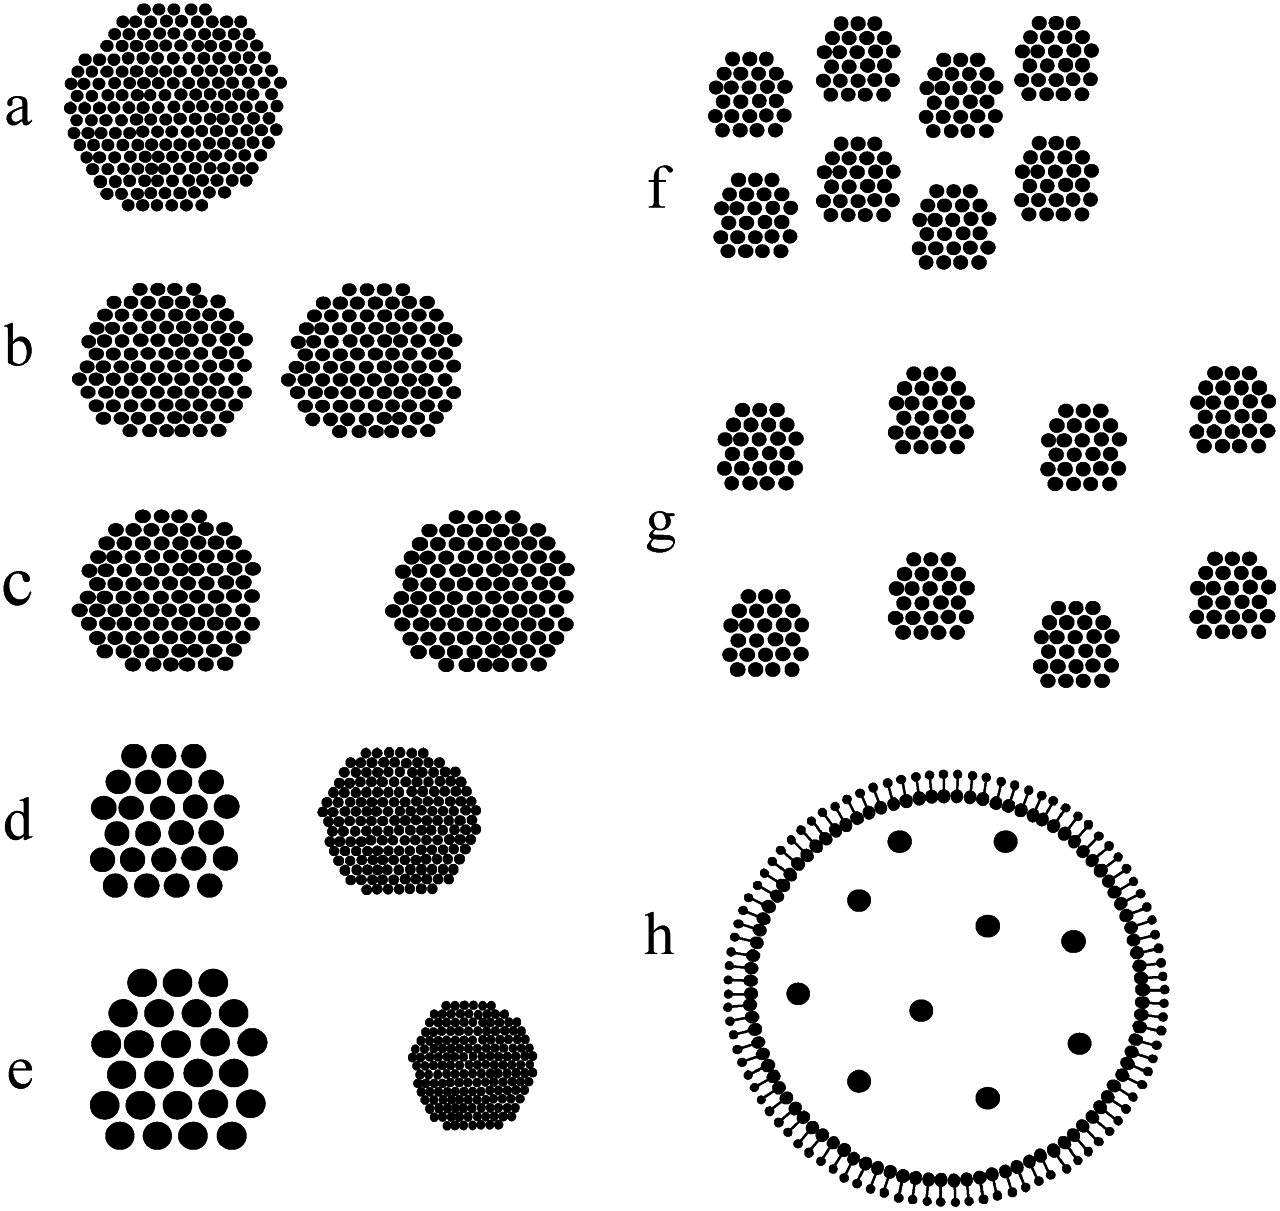
\includegraphics[height=0.8\textheight]{F1}}
\end{frame}

\begin{frame}{Simulations}
  \begin{enumerate}
    \setlength{\itemsep}{12pt}
    \item Network: use MCMC, adding and subtracting edges according to their
      log-likelihood.
    \item Epidemic: each sero-discordant partnership has a constant
      transmission rate.
    \item Viral evolution: coalescence rate for $n$ sequences of $n(n-1) /
      2N_eG$, where $N_e$ is the steady-state effective population size, and
      $G$ is viral the generation time. Also mutation rate $\mu_x$ for each
      site $x$.
  \end{enumerate}
\end{frame}

\begin{frame}{Prevalence varies across network types}
  \begin{columns}
    \begin{column}{0.5\textwidth}
      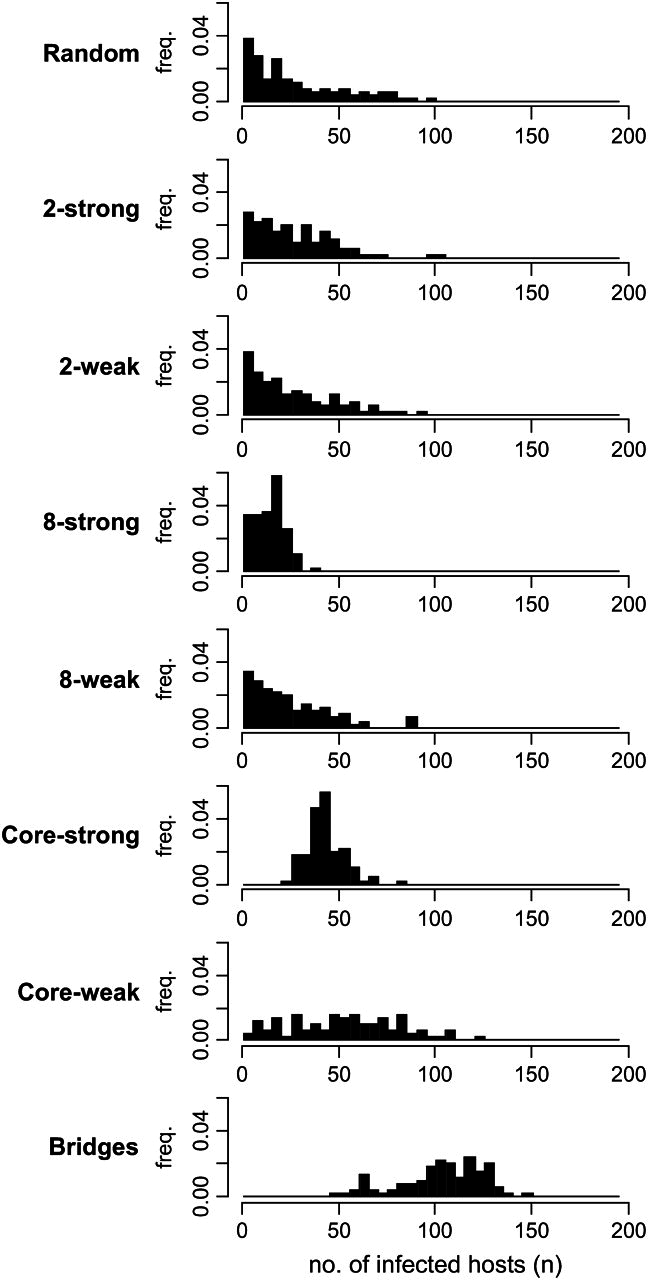
\includegraphics[width=\textwidth, trim=0 23cm 0 0, clip]{F2}
    \end{column}
    \begin{column}{0.5\textwidth}
      \vspace{0.5cm}
      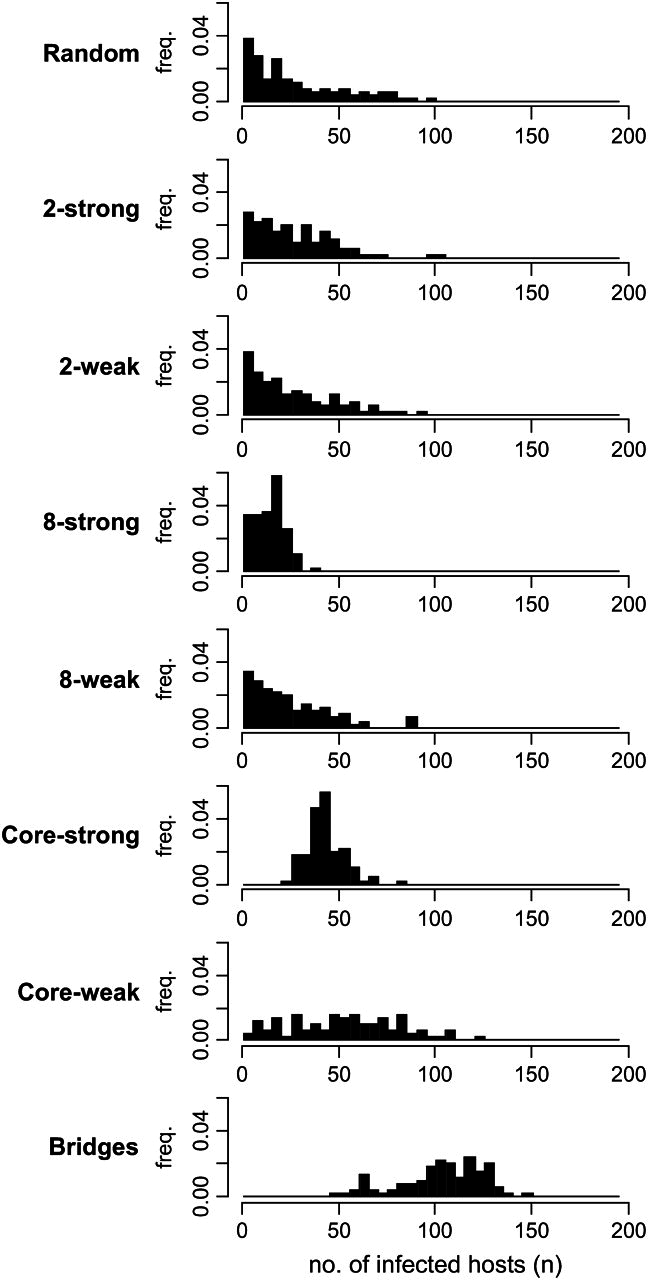
\includegraphics[width=\textwidth, trim=0 0 0 22cm, clip]{F2}
    \end{column}
  \end{columns}
\end{frame}

\begin{frame}{Simulations fall in expected range for random networks}
  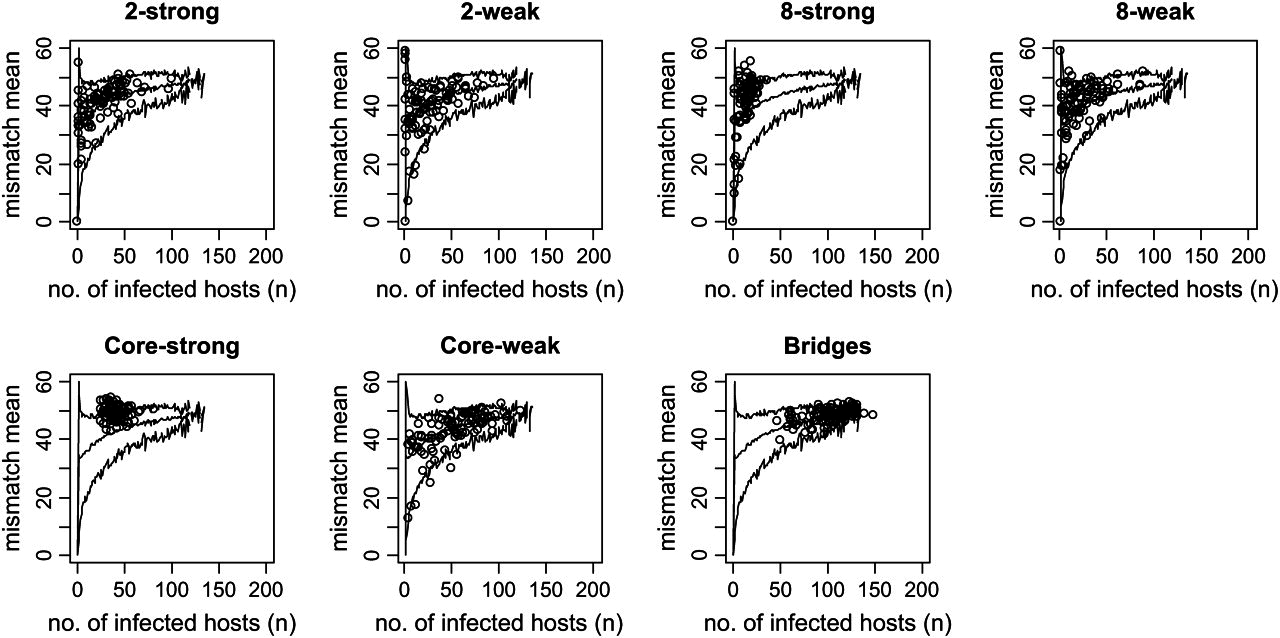
\includegraphics[width=\textwidth]{F3}

  Points are simulations, lines are expected values under panmixis.
\end{frame}

\begin{frame}{Most simulations best fit by exponential growth}
  \centerline{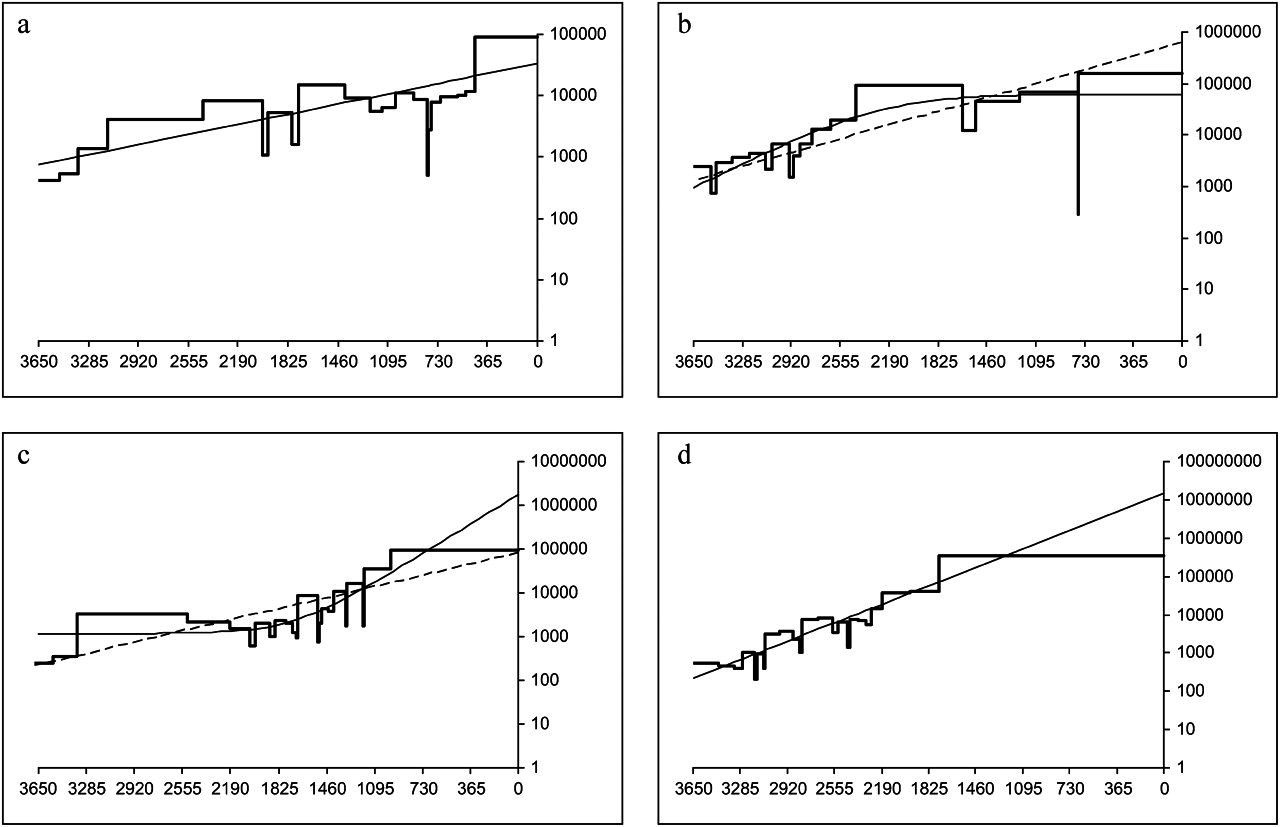
\includegraphics[height=2.5cm, trim=0 15cm 0 0, clip]{F4}}

  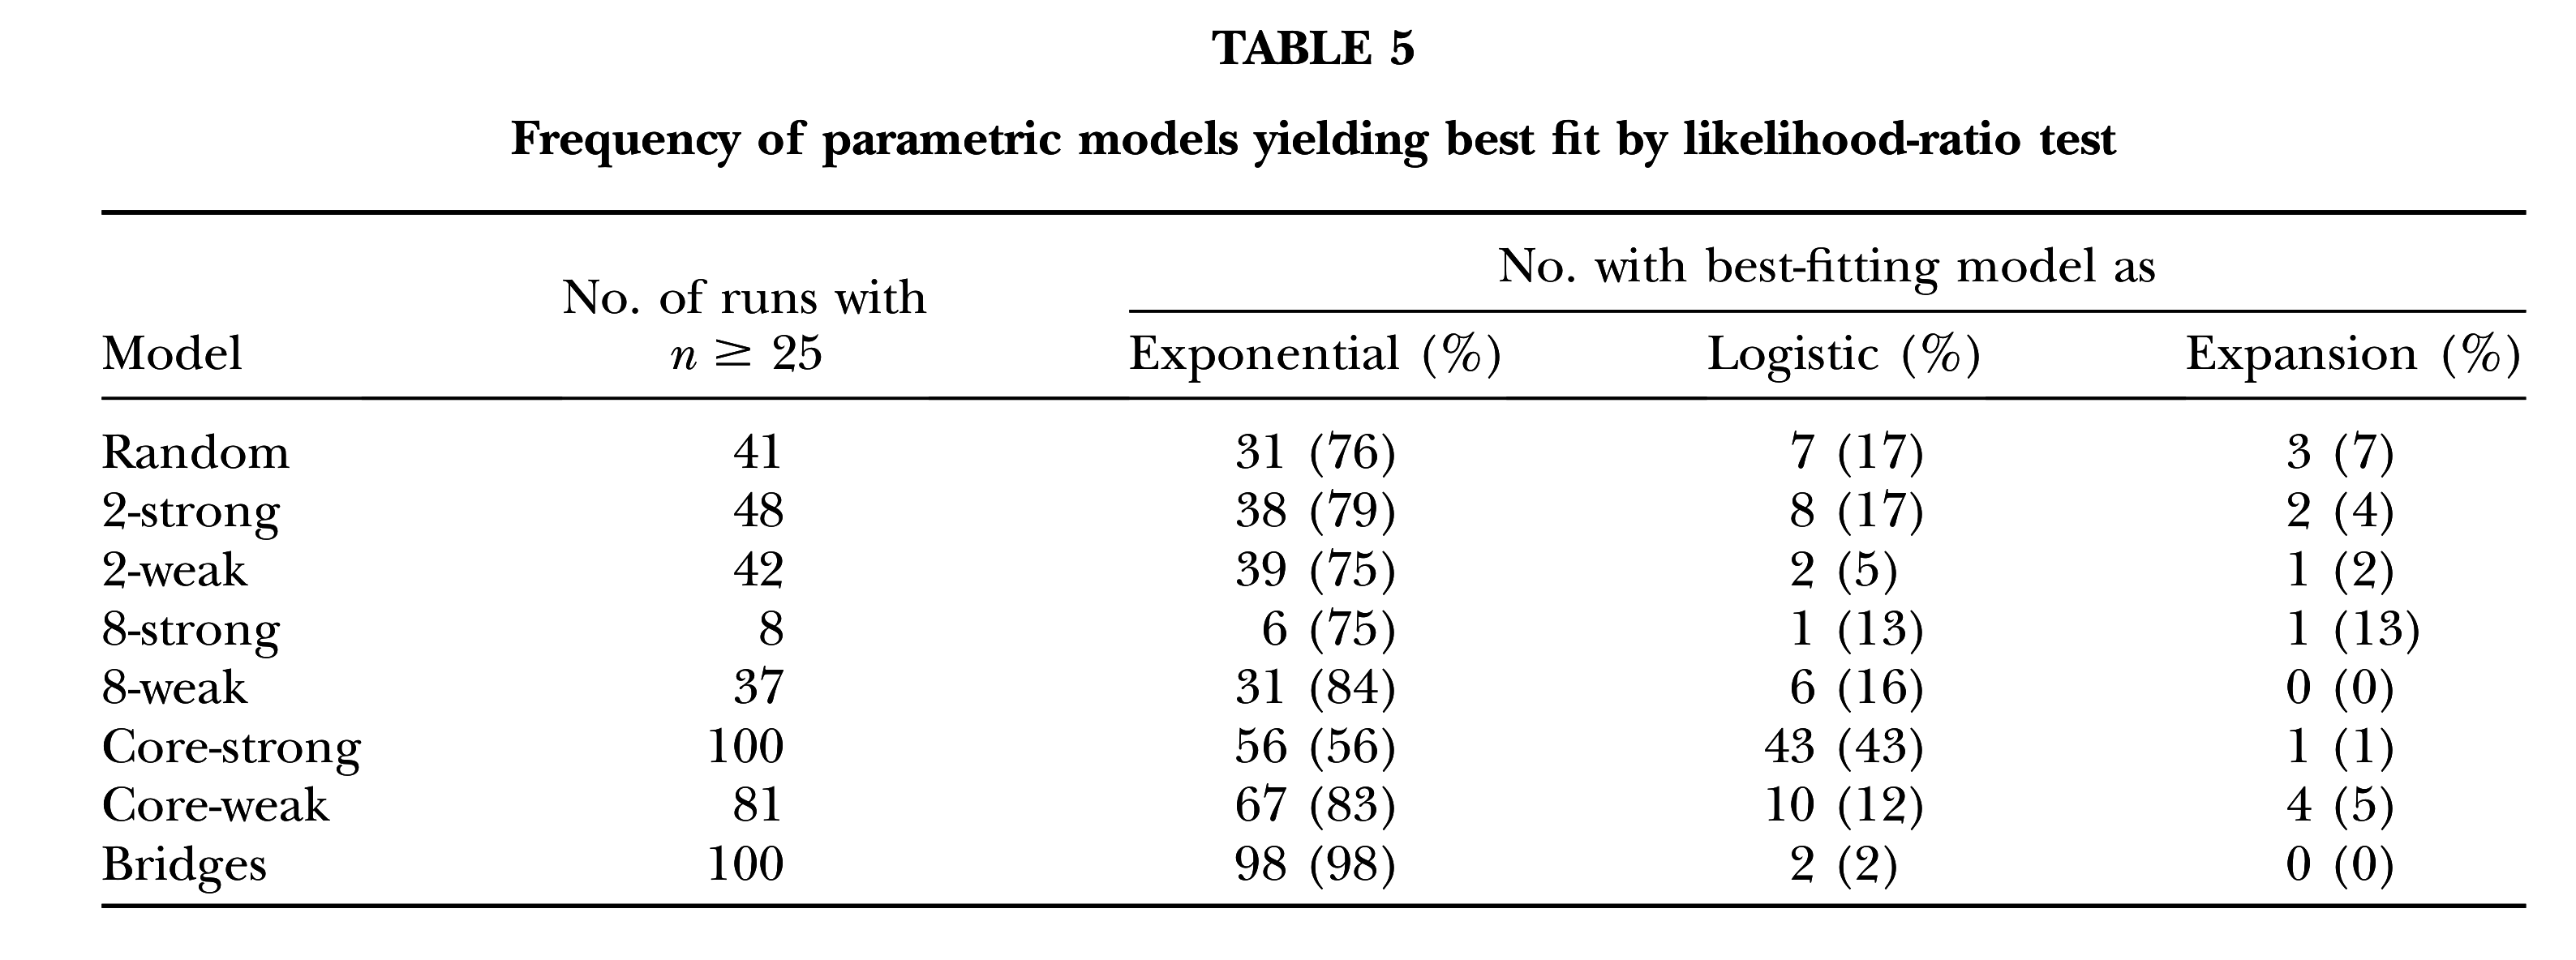
\includegraphics[width=\textwidth]{T5}
\end{frame}

\begin{frame}{Predicted and actual pop. size discrepancies}
  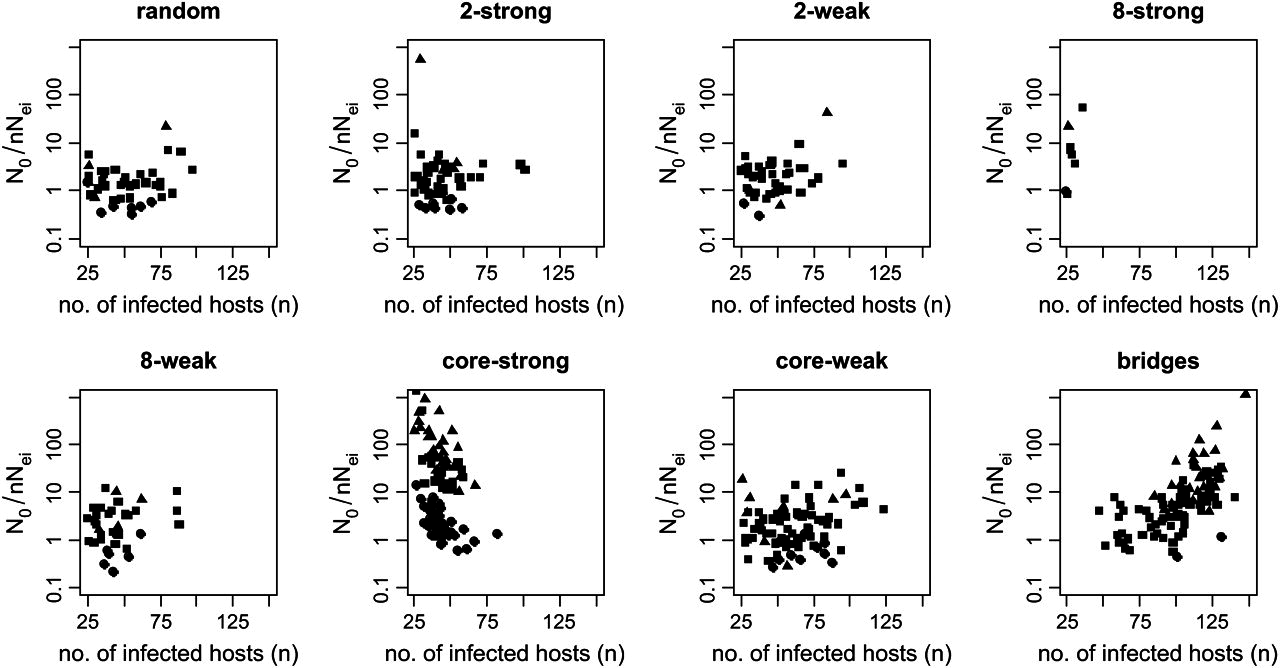
\includegraphics[width=\textwidth]{F5}
\end{frame}

\begin{frame}{Growth rate, pop. size may be over- or under-estimated}
  \begin{columns}
    \begin{column}{0.2\textwidth}
      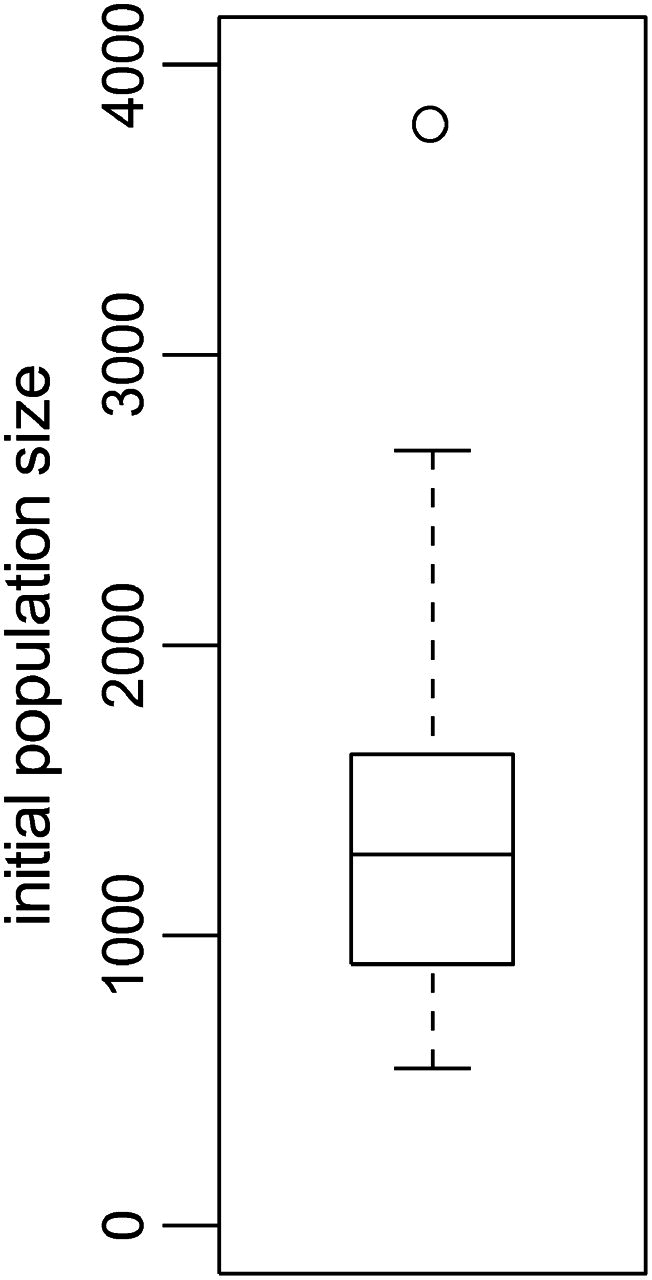
\includegraphics[width=\textwidth]{F6}
    \end{column}
    \begin{column}{0.7\textwidth}
      \vspace{0.5cm}
      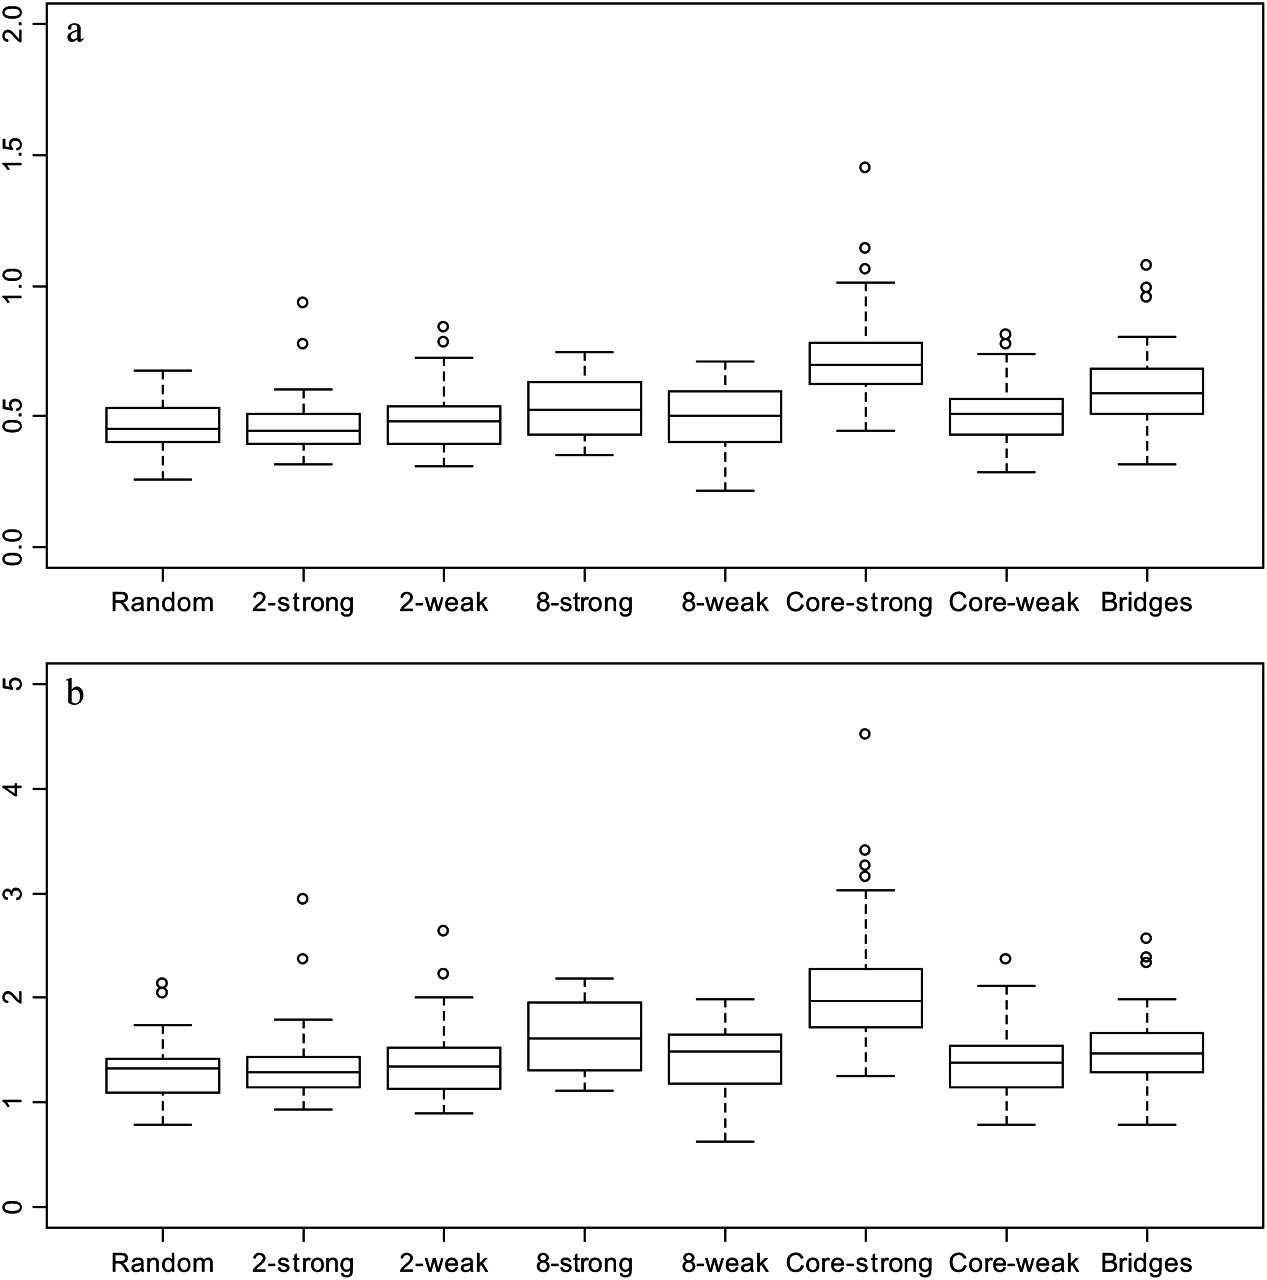
\includegraphics[height=0.8\textheight]{F7}
    \end{column}
  \end{columns}
\end{frame}

\end{document}
